\section{Project Management}
\begin{frame}{Project Management}
% \framesubtitle{Schedule}
    % \begin{minipage}{0.5\textwidth}
    %     % \setbeamertemplate{enumerate items}{\raisebox{-0.2em}{\scalebox{1.3}{\circled{\color{white}\insertenumlabel}}}}
    %     % \begin{enumerate}
    %     %     \itemsep1.3em
    %     %     \item Hadoop and MapReduce
    %     %     \item Apache Spark
    %     %     \item Spark SQL
    %     % \end{enumerate}
    %     This schedule was defined as part of the Specification document.
    % \end{minipage} \hfill
    % \begin{minipage}{0.49\textwidth}
    %     A particularly impactful element was the ``code freeze'' on Week 22.
        
    %     Sticking to this allowed me enough time to finish this presentation.
    %     % Otherwise it would not be done yet!
    % \end{minipage}
    \begin{wideitemize}
        \item Schedule defined as part of the Specification, planned for coding and writing reports.
        \item Code Freeze on Week 22 was very helpful
        \item Gave me enough time to finish the presentation!
    \end{wideitemize}
    
    \vfill\null
    \begin{tikzpicture}
        \node[inner sep=0pt] (gantt) at (0,0)
    {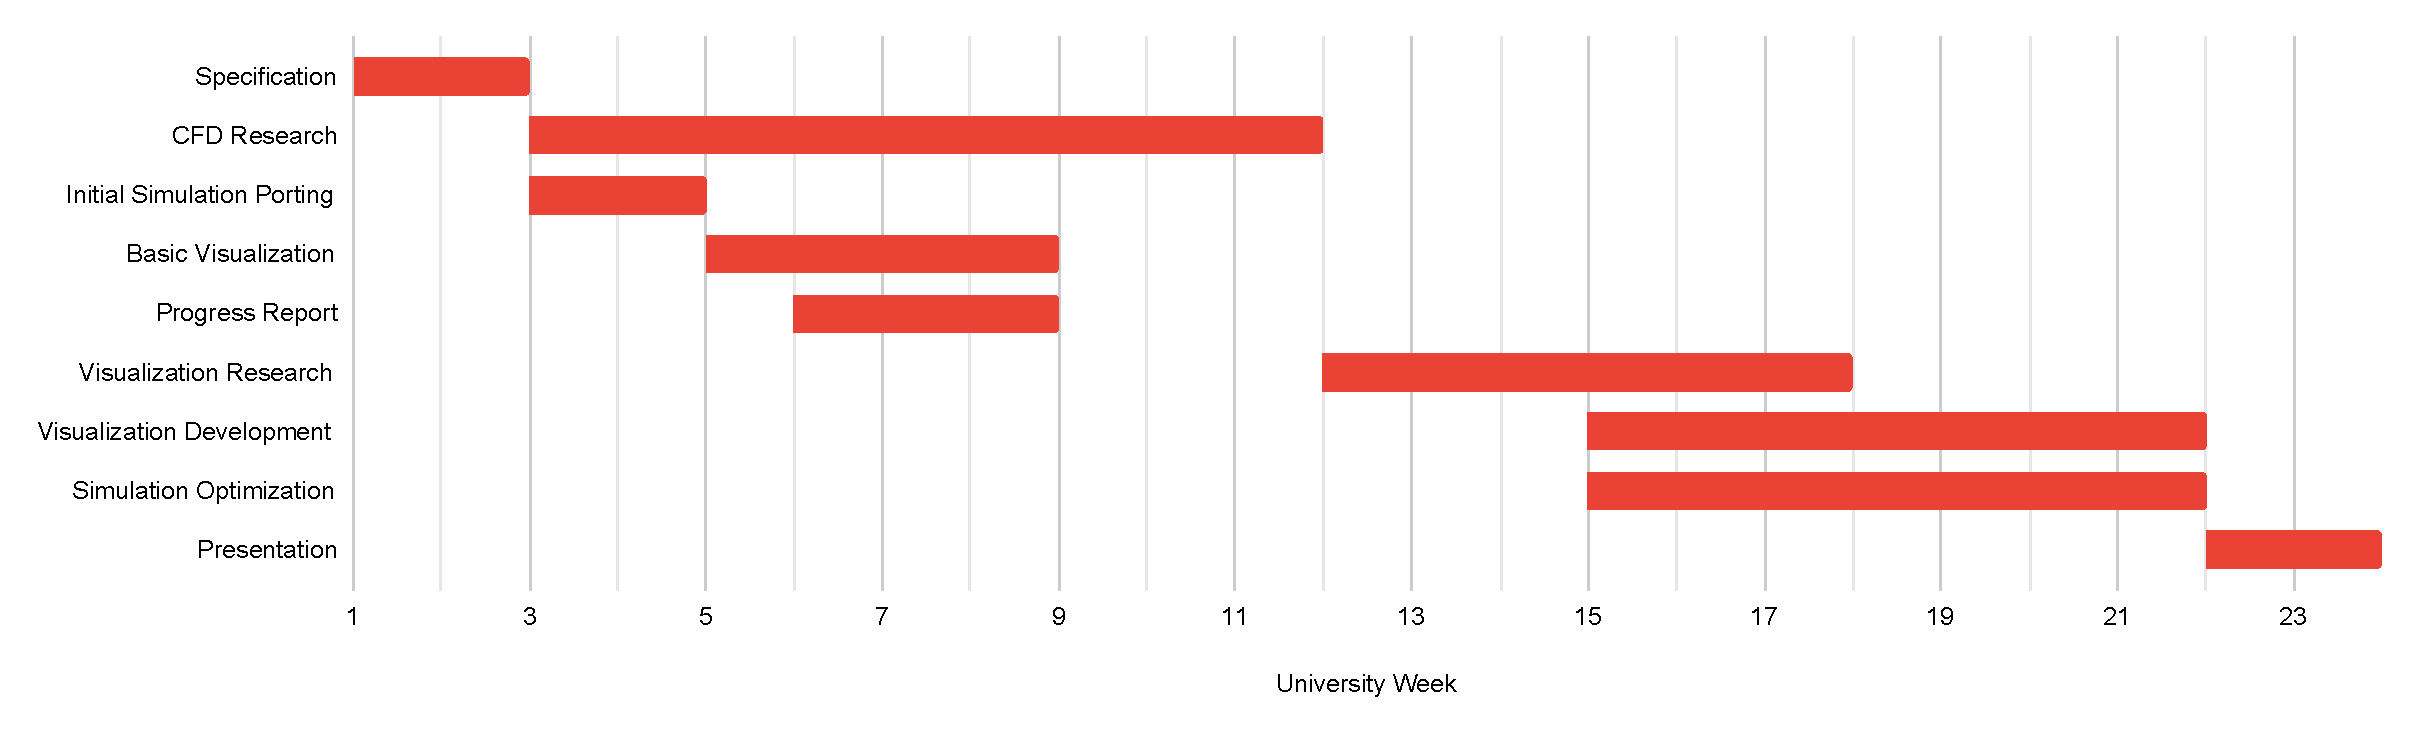
\includegraphics[width=1.0\linewidth]{Presentation/presentation_gantt.pdf}};
        \draw[line width=0.5mm] (5.4, -1.25) -- ++(0, 3) node[anchor=north east,align=right,fill=white] {Code Freeze};
        \node[text width=1.2cm,minimum height=2.35cm,fill opacity=0.5, fill=gray, font=\small,align=center, text opacity=1] at (-0.1,-0.02) {Christmas break and other work};
    \end{tikzpicture}
\end{frame}

% \begin{frame}{Project Management}
% \framesubtitle{Tools}
%     % C++17 + GCC 8
%     % CMake
%     % CUDA N
%     % vulkan.hpp
%     % Dear ImGui
%     % stb_image
% \end{frame}